\lhead[\thepage]{CHAPTER \thechapter. PLANNING AND BUDGET}
\chead[]{}
\rhead[A Complete Simulator for Volunteer Computing Environments\leftmark]{\thepage}
\renewcommand{\headrulewidth}{0.5pt}

\lfoot[]{}
\cfoot[]{}
\rfoot[]{}
\renewcommand{\footrulewidth}{0pt}

%% This is an example first chapter.  You should put chapter/appendix that you
%% write into a separate file, and add a line \include{yourfilename} to
%% main.tex, where `yourfilename.tex' is the name of the chapter/appendix file.
%% You can process specific files by typing their names in at the 
%% \files=
%% prompt when you run the file main.tex through LaTeX.
\chapter{Planificación y presupuesto}
\label{ch:planning_and_budget}
\markboth{}{PLANNING AND BUDGET}

This chapter presents a detailed planning of the project (Section \ref{sec:planning}, \textit{\nameref{sec:planning}}). Then, we explain the project costs (Section \ref{sec:budget}, \textit{\nameref{sec:budget}}). At the end of the chapter, we comment on the socio-economic environment of the project ({Section \ref{sec:socioeconomic_environment}, \textit{\nameref{sec:socioeconomic_environment}}}).

\section{Planificación}
\label{sec:planning}

This section includes the complete project planning. First, we describe the software development methodology used. After that, we detail the time duration of each phase of the project, collecting all times in a Gantt chart.

\subsection{Justificación de la Metodología}

Due to its characteristics, we have divided our project into three iterations:

\begin{itemize}

\item \textbf{Basic functionality:} the first iteration has been to achieve the simulation of a simple distributed computing system. The aim of this phase has been to simulate client machines that exchange messages with a server through the a network.

\item \textbf{Client side:} this phase has been to incorporate all the necessary functionality on the client side (described in Chapter \ref{ch:design}, \textit{\nameref{ch:design}}).

\item \textbf{Server side:} this phase has been to incorporate all the necessary functionality on the server side (described in Chapter \ref{ch:design}, \textit{\nameref{ch:design}}).

\end{itemize}

It was necessary to have an iterative methodology used to develop each of the phases independently to join all together in the last stage and obtain the final product. For this purpose, we have analyzed three different software development methodologies: Software prototyping \cite{grimm1998}, the Waterfall model \cite{hebert1983} and the Spiral model \cite{boehm1988}. Software prototyping did not fit well because it requires building a prototype of the software in a short time. The Waterfall model is a sequential design process, used in software development processes, in which progress is seen as flowing steadily downwards (like a waterfall) through different phases. The problem with this methodology is that it does not allow iterations within the software development. Finally, the Spiral model allowed fragmenting the project into different iterations. The model combines the strengths of the other two models (simplicity and flexibility), and uses an iterative process. Although this model is slower than the other two, it allowed us to apply different iterations so we decided to apply it to the whole process.

\subsection{Ciclo de Vida}

The life cycle development process of the project has followed the Spiral lifecycle model \cite{boehm1988}. Figure \ref{fig:spiral_model} shows the Spiral model using a scheme.

\begin{figure}[htbp]
 	\centering
 	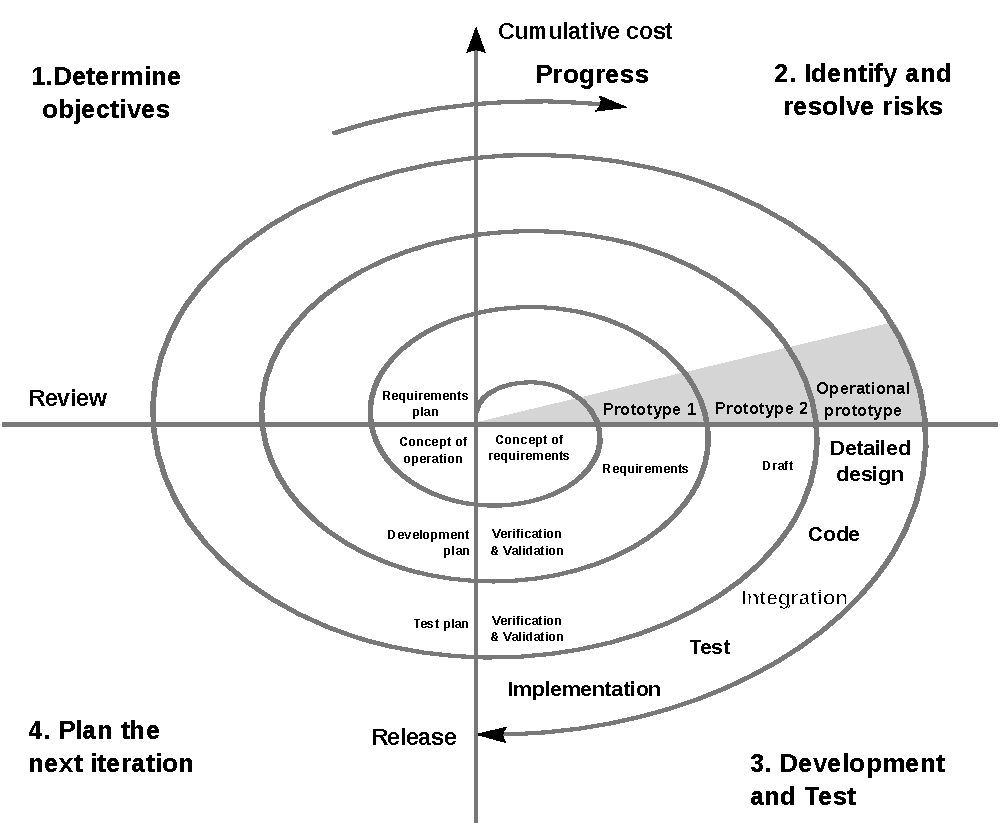
\includegraphics[width=12cm]{figures/spiral_model}
 	\caption{Spiral model (Boehm, 2000).}
	\label{fig:spiral_model}
\end{figure}

The Spiral model has four phases, which are repeated during the different iterations of the model. These phases are:

\begin{itemize}

\item \textbf{Planning} (Determine objectives in Figure \ref{fig:spiral_model}): the user requirements are gathered, a feasibility study of the system is performed, and the iteration objectives are determined. 

\item \textbf{Analysis} (Identify and resolve risks in Figure \ref{fig:spiral_model}): a full analysis of requirements is done and the potential risks are identified. This phase ends with a basic design.

\item \textbf{Development and Test}: Code implementation is done. Test cases and test results are performed.

\item \textbf{Evaluation} (Plan the next iteration in Figure \ref{fig:spiral_model}): Customers evaluate the software and provide their feedback. In this case, the student tries to get the supervisor's approval. This is  the \textit{critical task} of the life cycle, since we can only move on to the next iteration of the Spiral lifecycle model if this task is approved.

\end{itemize}

Each phase starts with a design goal and ends with the customer (the supervisor) reviewing the progress so far. As previously explained, we have divided the software development into three iterations: basic functionality, client side, and server side. In the last iteration, the complete software must undergo extensive testing in order to validate the simulator.


\subsection{Tiempo Estimado}

The Gantt chart (Figure \ref{fig:gantt}) shows all the tasks carried out during the project development. This project has been developed within a Collaboration in University Departments Scholarship \cite{colaboracion}, funded by the Spanish Ministry of Education, Culture, and Sport. The project began on November 2st, 2015, and ended on June 22, 2016, making a total of almost eight months of work. During this time, I have worked from Monday to Friday, four hours a day.

The Gantt chart shows all the tasks performed in each iteration of the spiral lifecycle model. Recall that the three iterations were: Basic functionality, Client side and Server side. In addition to the tasks (phases) mentioned above (Planning, Analysis, Development and Test, and Evaluation), we have included the Documentation task at the end of each iteration. The Documentation task has consisted mainly in drafting this bachelor thesis.


\begin{figure}[htbp]
 	\centering
 	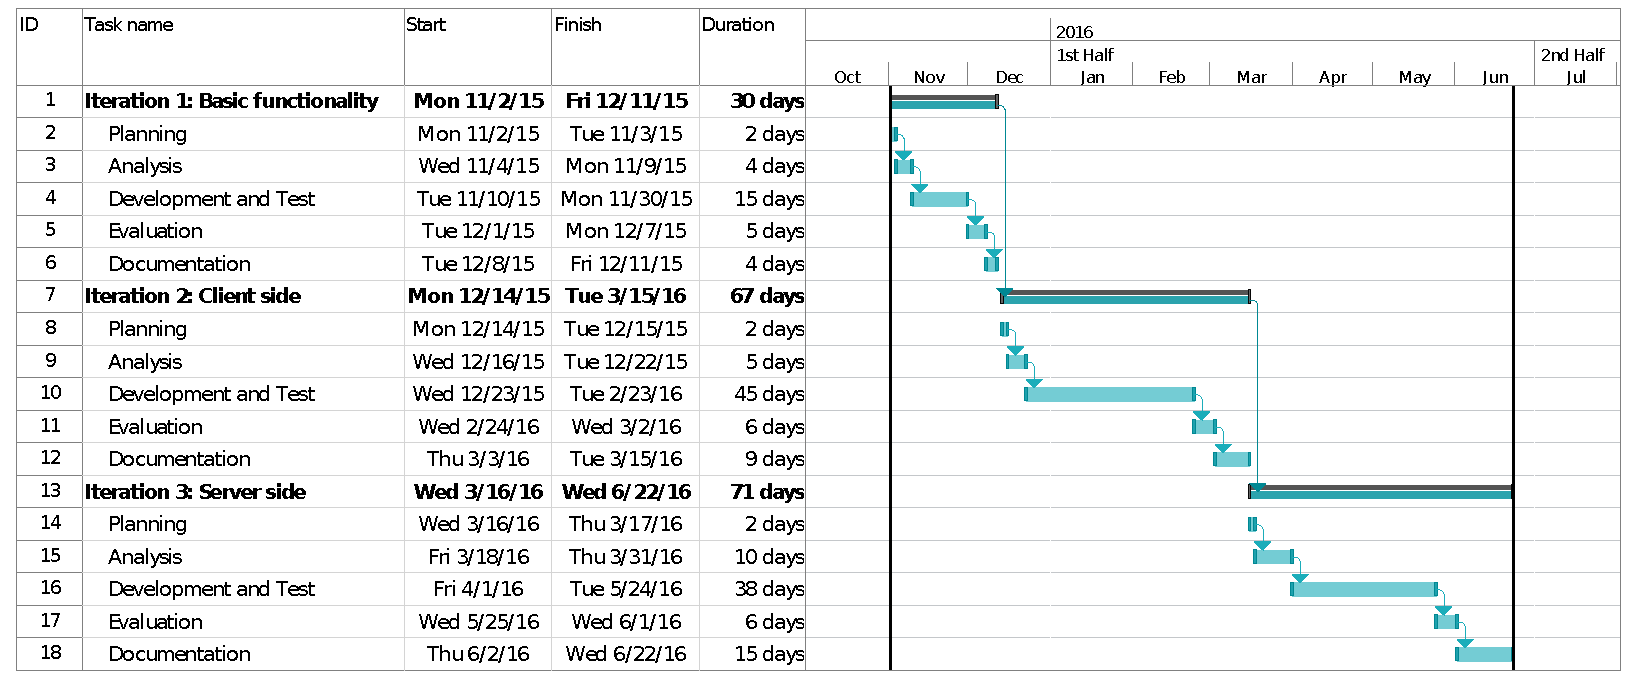
\includegraphics[width=16.5cm]{figures/gantt}
 	\caption{Gantt chart.}
	\label{fig:gantt}
\end{figure}

\section{Presupuesto}
\label{sec:budget}

This section details the overall project budget. On the one hand, we present the project costs and, on the other hand, we disclose the offer presented to the customer.

\subsection{Coste del Proyecto}

Table \ref{tab:project_information} summarizes the main features of the project including the total budget. 

\begin{center}
\ra{1.2}
\begin{table*}[htbp]
\centering
\begin{tabular}{@{}p{3.5cm} p{9cm}@{}} 
\toprule
\multicolumn{2}{c}{\textbf{\textit{Project Information}}}\\
\midrule
\textbf{Title} 					& A Complete Simulator for Volunteer Computing Environments \\
\midrule
\textbf{Author} 					& Saúl Alonso Monsalve \\
\midrule
\textbf{Department} 				& Computer Science and Engineering Department \\
\midrule
\textbf{Start date}				& 2nd of November of 2015 \\
\midrule
\textbf{End date}				& 22nd of June of 2016 \\
\midrule
\textbf{Duration} 				& 8 months \\
\midrule
\textbf{Indirect costs ratio} 	& 20 \% \\
\midrule
\textbf{Total budget} 			& 30,526.49 \\
\bottomrule
\end{tabular}
\caption{Project Information.}
\label{tab:project_information}
\end{table*}
\end{center}

Then the total budget of the project is broken down below.

\subsubsection{Costes Directos}

In this part, the direct costs of the project are presented. Table \ref{tab:dhrc} shows the direct costs caused by personnel costs, based on the planning presented in the previous section. The supervisor and the student have played the following roles:

\begin{itemize}

\item \textbf{Supervisor:} Project manager.

\item \textbf{Student:} Analyst, Developer, Tester.

\end{itemize} 

\begin{center}
\ra{1.2}
\begin{table*}[htbp]
\centering
\begin{tabular}{@{}p{3cm} R{3.5cm} R{2.2cm} R{2.4cm}@{}} 
\toprule
\textbf{Category} & \textbf{Cost per hour (\euro)} & \textbf{Hours} & \textbf{Total (\euro)} \\
\midrule
Project manager					& 60 						& 56			& 3,360 \\
Analyst			 				& 35							& 188		& 6,580 \\
Developer		 				& 35							& 316		& 11,060 \\
Tester		 					& 25							& 112		& 2,800 \\
\midrule
\textbf{\textit{Total}}			&							&			& \textbf{23,800.00}\\
\bottomrule
\end{tabular}
\caption{Human resources costs.}
\label{tab:dhrc}
\end{table*}
\end{center}

Table \ref{tab:dec} shows the direct costs caused by equipment acquisition and usage. The chargeable cost, C, is calculated using the following formula:

\begin{equation}
  C = \frac{d \cdot c \cdot u}{D}
\label{eq:costs}
\end{equation}

Where:

\begin{itemize}

\item \textbf{C:} Chargeable cost. It is equivalent to the depreciated value.

\item \textbf{d:} Time the equipment has been used.

\item \textbf{c:} Equipment cost. 

\item \textbf{u:} Project dedication. Percentage of time the equipment has been used.

\item \textbf{D:} Equipment depreciation period.

\end{itemize}

\begin{center}
\ra{1.2}
\begin{table*}[htbp]
\centering
\begin{tabular}{@{}p{2.5cm} C{1.8cm} C{2.1cm} C{2.1cm} C{2.7cm} C{2.3cm}@{}} 
\toprule
\textbf{Concept} & \textbf{Cost, c (\euro)} & \textbf{Dedication, u (\%)} & \textbf{Dedication, d (months)} & \textbf{Depreciation, D (months)} & \textbf{Chargeable cost, C (\euro)}\\
\midrule
Desktop \acrshort{pc}		 			& \multicolumn{1}{r}{799.99}		& \multicolumn{1}{r}{100}		& \multicolumn{1}{r}{8} 		& 	\multicolumn{1}{r}{36}	& 	\multicolumn{1}{r}{177.78} \\
Laptop 						& \multicolumn{1}{r}{529.99} 	& \multicolumn{1}{r}{25}			& \multicolumn{1}{r}{8} 		& 	\multicolumn{1}{r}{36}	& 	\multicolumn{1}{r}{29.44} \\
\acrshort{arcos} Tucan					& \multicolumn{1}{r}{89,501.60}	& \multicolumn{1}{r}{10}			& \multicolumn{1}{r}{6} 		& 	\multicolumn{1}{r}{60}	& 	\multicolumn{1}{r}{895.02} \\
\acrshort{arcos} Mirlo					& \multicolumn{1}{r}{2,469.99}	& \multicolumn{1}{r}{70}			& \multicolumn{1}{r}{6} 		& 	\multicolumn{1}{r}{60}	& 	\multicolumn{1}{r}{172.90} \\
Printer						& \multicolumn{1}{r}{399.24}		& \multicolumn{1}{r}{5}			& \multicolumn{1}{r}{3}		& 	\multicolumn{1}{r}{60}	& 	\multicolumn{1}{r}{1.00} \\
\midrule
\textbf{\textit{Total}}		&			&			& 			& &  \multicolumn{1}{r}{\textbf{1,276.14}}\\
\bottomrule
\end{tabular}
\caption{Equipment costs.}
\label{tab:dec}
\end{table*}
\end{center}

Furthermore, the equipment presented in Table \ref{tab:dec} is detailed below:

\begin{itemize}

\item \textbf{Desktop \acrshort{pc}:} All in One - Asus Z220ICUK, 21.5'', i5-6400T, 8GB, 1TB)		

\item \textbf{Laptop:} Toshiba L50D-C-19D, A10-8700P, 8GB \gls{ram} and 1TB.

\item \textbf{\acrshort{arcos} Tucan:} Cluster used by the research group \acrshort{arcos}.

\item \textbf{\acrshort{arcos} Mirlo:} Server used by the research group \acrshort{arcos}. 32GB \gls{ram} and eight i7 processors of 2.67GHz each.

\item \textbf{Printer:} HP LaserJet Enterprise P3015.

\end{itemize}

Other direct costs are shown in Table \ref{tab:odc}. These costs consist of office material, a toner for the printer, and the monthly travel pass. Office material includes: pencils, pens, notebooks, paper, tipex, and markers.

\begin{center}
\ra{1.2}
\begin{table*}[htbp]
\centering
\begin{tabular}{@{}p{5cm} R{3.5cm}@{}} 
\toprule
\textbf{Concept} & \textbf{Cost (\euro)} \\
\midrule
Office material					& 112.98				\\
Toner (x1) 			 			& 89.62				\\
Monthly travel pass (x8) 		& 160				\\
\midrule
\textbf{\textit{Total}}			& \textbf{362.60} 	\\
\bottomrule
\end{tabular}
\caption{Other direct costs.}
\label{tab:odc}
\end{table*}
\end{center}

\subsubsection{Resumen de Costes}

Table \ref{tab:cs} shows the complete summary of the project costs. Indirect costs (20\% of direct costs) consist of the electricity and water bills, telephone, Internet access, etc.

\begin{center}
\ra{1.2}
\begin{table*}[htbp]
\centering
\begin{tabular}{@{}p{5cm} R{5cm}@{}} 
\toprule
\multicolumn{2}{c}{\textbf{\textit{Costs summary}}}\\
\midrule
\textbf{Human resources} 				& 23,800.00 \\
\textbf{Equipment} 						& 1,276.14 \\
\textbf{Other direct costs} 				& 362.60 \\
\textbf{Indirect costs}					& 5,087.75 \\
\midrule
\textbf{\textit{Total budget}}			& \textbf{30,526.49} \\
\bottomrule
\end{tabular}
\caption{Costs summary.}
\label{tab:cs}
\end{table*}
\end{center}

The total budget for this project amounts to \textbf{30,526.49 \euro \ (thirty thousand five hundred twenty-six euro and forty-nine cent)}.

\subsection{Oferta de Proyecto Propuesta}

Table \ref{tab:offer} shows a detailed offer proposal. This offer includes the estimated risks (20\%), the expected benefits (15\%), and the Value Added Tax (Spanish \gls{iva}), which corresponds to 21\% \cite{iva2012}. After applying all theses concepts, the final amount for this project in case of sale to a third-party client is \textbf{50,973.14 \euro \ (fifty thousand nine hundred seventy-three euro and fourteen cent).}

\begin{center}
\ra{1.2}
\begin{table*}[htbp]
\centering
\begin{tabular}{@{}p{2.5cm} R{2.6cm} R{3.1cm} R{3.5cm}@{}} 
\toprule
\multicolumn{4}{c}{\textbf{\textit{Offer proposal}}}\\
\midrule
\textbf{Concept} & \textbf{Increment (\%)} & \textbf{Partial value (\euro)} & \textbf{Aggregated cost (\euro)} \\
\midrule
Project costs				& - 			& 30,526.49		& 30,526.49 \\
Risk			 				& 20			& 6,105.30		& 36,631.79 \\
Benefits		 				& 15			& 5,494.77		& 42,126.56 \\
IVA		 					& 21			& 8,846.58		& 50,973.14 \\
\midrule
\textbf{\textit{Total}}		&			&			& \textbf{50,973.14}\\
\bottomrule
\end{tabular}
\caption{Offer proposal.}
\label{tab:offer}
\end{table*}
\end{center}

\section{Entorno Socio-Económico}
\label{sec:socioeconomic_environment}

As commented in previous chapters, \gls{comsimboinc} can guide the design of \gls{boinc} projects. This means that \gls{boinc} project designers can perform accurate simulations using \gls{comsimboinc} before deploying the system. Thanks to this, designers can save money and resources, because they will know the performance of the system before deploying it. In addition, it can also save energy because designers will not need to perform tests using the original infrastructure, as they will only need to use \gls{comsimboinc} in order to analyze the functioning of different alternatives.

Moreover, \gls{boinc} operates as a platform for distributed applications in areas as diverse as mathematics, medicine, molecular biology, climatology, environmental science, and astrophysics. On the one hand, there are projects that help the scientific community, such as the SETI@home project \cite{Anderson2002SETI@home}, of which the purpose is to analyze radio signals, searching for signs of extraterrestrial intelligence; or the Citizen Science Grid project \cite{csgproject}, which is dedicated to supporting a wide range of research and educational projects. On the other hand, there are projects dedicated to the environmental care, such as the Climateprediction.net project \cite{climateprediction}, which studies climate. Therefore, our simulator indirectly contributes to both science and the environment.


